\documentclass[10pt,fleqn]{article}
\usepackage{hyperref}
\usepackage{graphicx}


\setlength{\topmargin}{-.75in}
\addtolength{\textheight}{2.00in}
\setlength{\oddsidemargin}{.00in}
\addtolength{\textwidth}{.75in}

\nofiles

\pagestyle{empty}

\setlength{\parindent}{0in}

% new math commands


\setlength{\oddsidemargin}{-0.25in}
\setlength{\evensidemargin}{-0.25in}
\setlength{\textwidth}{6.75in}
\setlength{\headheight}{0.0in}
\setlength{\topmargin}{-0.25in}
\setlength{\textheight}{9.00in}

\makeindex

\usepackage{mathrsfs}

%\usepackage[pdftex]{graphicx}
\usepackage{epstopdf}

\newcounter{beans}

\newcommand{\ds}{\displaystyle}
\newcommand{\limit}[2]{\displaystyle\lim_{#1\to#2}}

\newcommand{\binomial}[2]{\ \left( \begin{array}{c}
                                  #1 \\
                                  #2
                                 \end{array}
                            \right) \
                         }
\newcommand{\ExampleRule}[2]
  {
  \noindent
  \rule{\linewidth}{1pt}
  \begin{example}
    #1
    \label{#2}
  \end{example}
  \rule{\linewidth}{1pt}
  \vskip0.125in
  }

\newcommand{\defbox}[1]
  {
   \ \\
   \noindent
   \setlength\fboxrule{1pt}
   \fbox{
        \begin{minipage}{6.5in}
          #1
        \end{minipage}
        }
   \ \\
  }
\newcommand{\verysmallworkbox}[1]
  {
   \ \\
   \noindent
   \setlength\fboxrule{1pt}
   \fbox{
        \begin{minipage}{6.5in}
           #1
           \ \\
           \vskip0.5in \ \\
           \ \\
        \end{minipage}
        }
   \ \\
  }
\newcommand{\smallworkbox}[1]
  {
   \ \\
   \noindent
   \setlength\fboxrule{1pt}
   \fbox{
        \begin{minipage}{6.5in}
           #1
           \ \\
           \vskip2.5in \ \\
           \ \\
        \end{minipage}
        }
   \ \\
  }
\newcommand{\halfworkbox}[1]
  {
   \ \\
   \noindent
   \setlength\fboxrule{1pt}
   \fbox{
        \begin{minipage}{6.5in}
           #1 \hfill
           \ \\
           \vskip3.25in \ \\
           \ \\
        \end{minipage}
        }
   \ \\
  }
\newcommand{\largeworkbox}[1]
  {
   \ \\
   \noindent
   \setlength\fboxrule{1pt}
   \fbox{
        \begin{minipage}{6.5in}
           #1
           \ \\
           \vskip7.5in \ \\
           \ \\
        \end{minipage}
        }
   \ \\
  }
\newcommand{\flexworkbox}[2]
  {
   \ \\
   \noindent
   \setlength\fboxrule{1pt}
   \fbox{
        \begin{minipage}{6.5in}
           #1
           \ \\

           \vskip#2 \ \\
           \ \\
        \end{minipage}
        }
   \ \\
  }


% symbols for sets of numbers

\newcommand{\natnumb}{$\cal N$}
\newcommand{\whonumb}{$\cal W$}
\newcommand{\intnumb}{$\cal Z$}
\newcommand{\ratnumb}{$\cal Q$}
\newcommand{\irrnumb}{$\cal I$}
\newcommand{\realnumb}{$\cal R$}
\newcommand{\cmplxnumb}{$\cal C$}

% misc. commands

\newcommand{\mma}{{\it Mathematica}}
\newcommand{\sech}{\mbox{ sech}}
 
\newtheorem{theorem}{Theorem}
\newtheorem{example}{Example}
\newtheorem{definition}{Definition}
\newtheorem{problem}{Problem}

\setcounter{secnumdepth}{2}
\setcounter{tocdepth}{4}


\begin{document}
%%%%%%%%%%%%%%%%%%%%%%%%%%%%%%%%%%%%%%%%%%%%%%%%%%%%%%%%%%%%%%%%%%%%%%%%%%%%%%%%
%%%%%%%%%%%%%%%%%%%%%%%%%%%%%%%%%%%%%%%%%%%%%%%%%%%%%%%%%%%%%%%%%%%%%%%%%%%%%%%%
\vskip0.1in\hrule\vskip0.1in \noindent
{\bf Math 4610 Fundamentals of Computational Mathematics  - Topic 8.}
\vskip0.1in\hrule\vskip0.1in \noindent
%%%%%%%%%%%%%%%%%%%%%%%%%%%%%%%%%%%%%%%%%%%%%%%%%%%%%%%%%%%%%%%%%%%%%%%%%%%%%%%%
%%%%%%%%%%%%%%%%%%%%%%%%%%%%%%%%%%%%%%%%%%%%%%%%%%%%%%%%%%%%%%%%%%%%%%%%%%%%%%%%
\vskip0.1in\hrule\vskip0.1in\noindent\noindent
{\bf Using git to Work Locally on Your Computer} 
\vskip0.1in\hrule\vskip0.1in\noindent
You can chose to work on projects on Github by logging onto the Github web site.
However, if your internet connection is not as good as you might like, you can
use \lq\lq git\rq\rq\ to synchronize the work on your project. The git
environment is a Version Control System (VCS) which allows different groups to
work on the same project without stepping on each other's toes. In this topic
we will learn a bit about git and start using git to synchronize your work on
Github. Your work will be downloaded from Github for grading. 
%%%%%%%%%%%%%%%%%%%%%%%%%%%%%%%%%%%%%%%%%%%%%%%%%%%%%%%%%%%%%%%%%%%%%%%%%%%%%%%%
%%%%%%%%%%%%%%%%%%%%%%%%%%%%%%%%%%%%%%%%%%%%%%%%%%%%%%%%%%%%%%%%%%%%%%%%%%%%%%%%
\vskip0.1in\hrule\vskip0.1in\noindent\noindent
{\bf Using git to Work Locally on Your Computer} 
\vskip0.1in\hrule\vskip0.1in\noindent
The first thing to do is to make sure that git is available within your terminal
or terminal emulator. To do this use the following command:
\begin{verbatim}

    koebbe% which git

\end{verbatim}
If git is available, you will see output like that in the following figure. In
this case, the executable for git is in the folder /usr/bin. If git is not
available, you can install the software on most computers. If you need some help
getting the sofware installed, talk to your instructor.
\vfill
\begin{figure}[h]
\centering
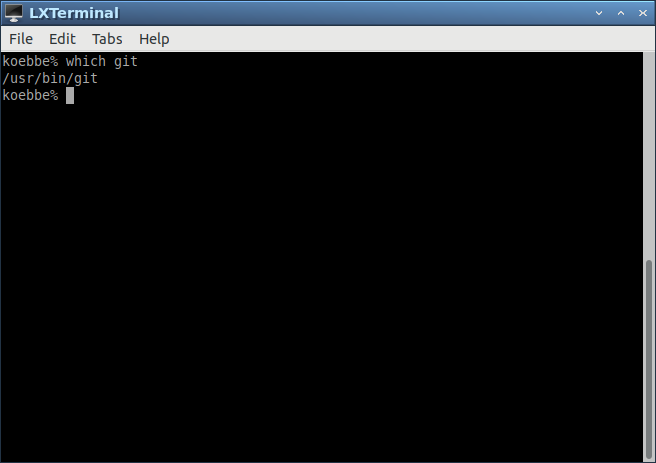
\includegraphics{../images/git_01.png}
\vskip0.1in
\caption{Checking for git using the which command.}
\end{figure}
\eject
%%%%%%%%%%%%%%%%%%%%%%%%%%%%%%%%%%%%%%%%%%%%%%%%%%%%%%%%%%%%%%%%%%%%%%%%%%%%%%%%
%%%%%%%%%%%%%%%%%%%%%%%%%%%%%%%%%%%%%%%%%%%%%%%%%%%%%%%%%%%%%%%%%%%%%%%%%%%%%%%%
\vskip0.1in\hrule\vskip0.1in\noindent
{\bf Command in the git VCS} 
\vskip0.1in\hrule\vskip0.1in\noindent
This section of notes will not cover all possible ways to use and modify git.
Instead, we will look at some basic commands that git uses to share the data in
a repository. The general form for a command using git is the following:
\begin{verbatim}

    % git command [options]

\end{verbatim}
To start, we can type in the command
\begin{verbatim}

    koebbe% git --help

\end{verbatim}
This produces a couple of screens of output. Another way to display the same
output, one screen at a time, is to pipe the output from the command above into
another Unix command. The result is
\begin{verbatim}

    koebbe% git --help | more

\end{verbatim}
The concept of a pipe in Unix is to take the output from one command and use
this as input to another command. So, the output from
\begin{verbatim}

    koebbe% git --help

\end{verbatim}
is piped into the more command. The more command will display output one screen
at a time. You should try this some time.

What you should notice is all of the options for running commands within git.
The end result is that you can read the first screen and then hit a space bar
to read the next screen. The rest of this section of notes will go over a bare
minimum of git so that you can work on your own computer.
\vfill
\begin{figure}[h]
\centering
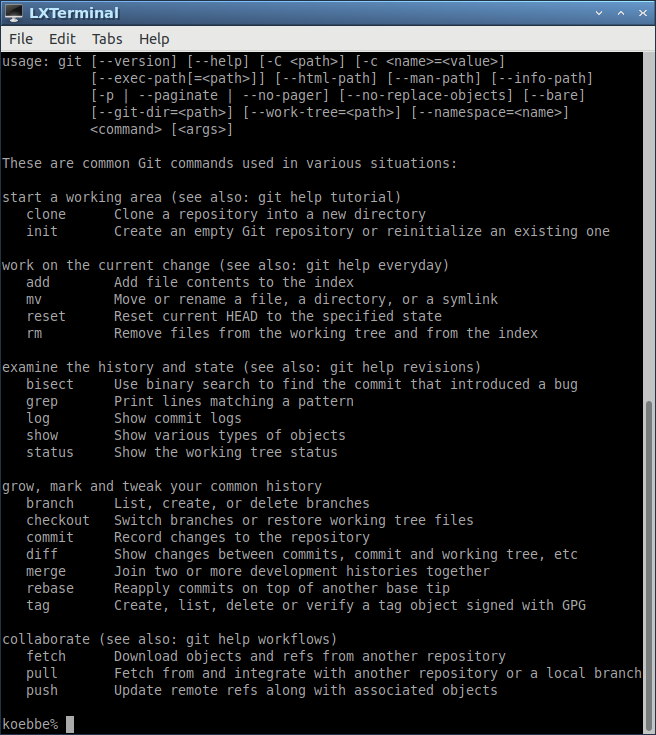
\includegraphics{../images/git_02.png}
\vskip0.1in
\caption{The first part of the output gives about half of the possible options
         we can use with git.}
\end{figure}
%\eject
\vfill
\begin{figure}[h]
\centering
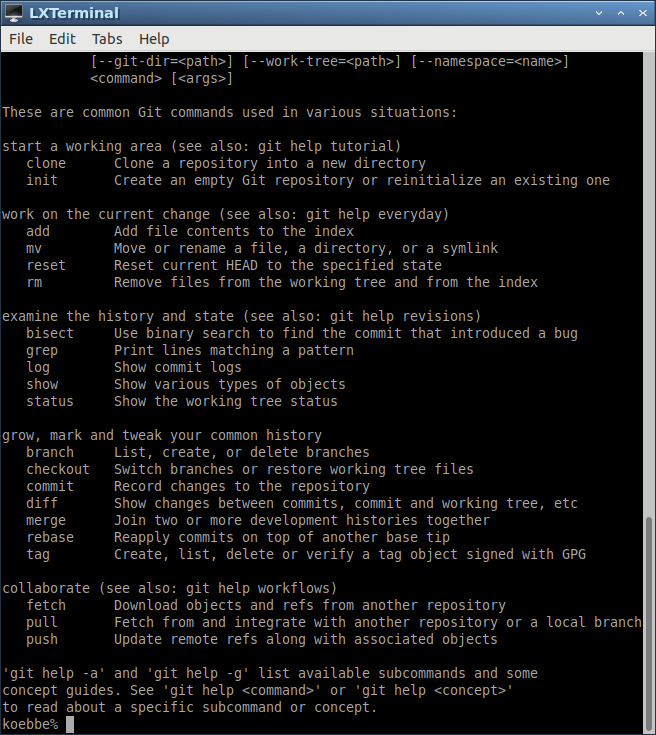
\includegraphics{../images/git_03.png}
\vskip0.1in
\caption{Checking for git using the which command.}
\end{figure}
\eject
%%%%%%%%%%%%%%%%%%%%%%%%%%%%%%%%%%%%%%%%%%%%%%%%%%%%%%%%%%%%%%%%%%%%%%%%%%%%%%%%
%%%%%%%%%%%%%%%%%%%%%%%%%%%%%%%%%%%%%%%%%%%%%%%%%%%%%%%%%%%%%%%%%%%%%%%%%%%%%%%%
\vskip0.1in\hrule\vskip0.1in\noindent
{\bf Initializing a Folder Using the git init} 
\vskip0.1in\hrule\vskip0.1in\noindent
To start, there are two ways to initialize a git folder. The first is to take
a new folder and initialize the folder using
\begin{verbatim}

    koebbe% mkdir tempdir
    koebbe% cd tempdir
    koebbe% git init

\end{verbatim}
As the output states, the result is an empty Git repository. The other method
will work well for making a copy of the Github repository named math4610. You
can clone a repository from another site. To do this, change into the folder
where the repository folder will end up.
\vfill
\begin{figure}[h]
\centering
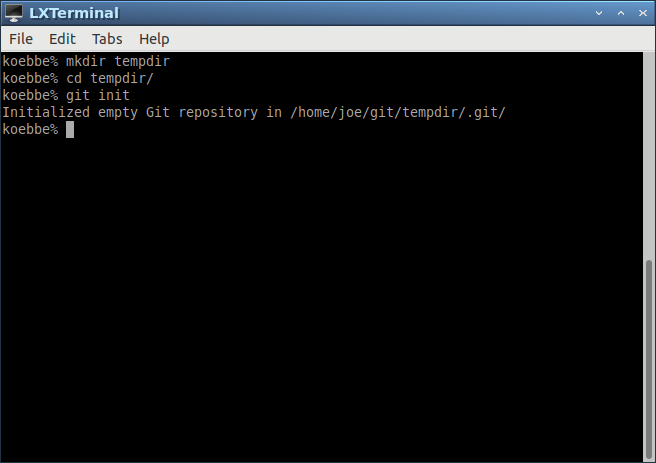
\includegraphics{../images/git_04.png}
\vskip0.1in
\caption{Creation of a local repository using the git init command.}
\end{figure}
\eject
%%%%%%%%%%%%%%%%%%%%%%%%%%%%%%%%%%%%%%%%%%%%%%%%%%%%%%%%%%%%%%%%%%%%%%%%%%%%%%%%
%%%%%%%%%%%%%%%%%%%%%%%%%%%%%%%%%%%%%%%%%%%%%%%%%%%%%%%%%%%%%%%%%%%%%%%%%%%%%%%%
\vskip0.1in\hrule\vskip0.1in\noindent
{\bf Initializing a Folder Using the git clone} 
\vskip0.1in\hrule\vskip0.1in\noindent
We can use the clone command in git.

To do this, type
\begin{verbatim}

    koebbe% cd foldername
    koebbe% git clone https://www.github.com/username/repositoryname

\end{verbatim}
So, if Fred has chosen fred as a username on Github, the pair of commands would
be
\begin{verbatim}

    koebbe% cd repository_location
    koebbe% git clone https://www.github.com/fred/math4610

\end{verbatim}
This will put a copy of everything in math4610 in a directory on your computer.
Note that in the figure below a different repository was used. The math4610
repository is too large and takes a bit of time to clone.
\vfill
\begin{figure}[h]
\centering
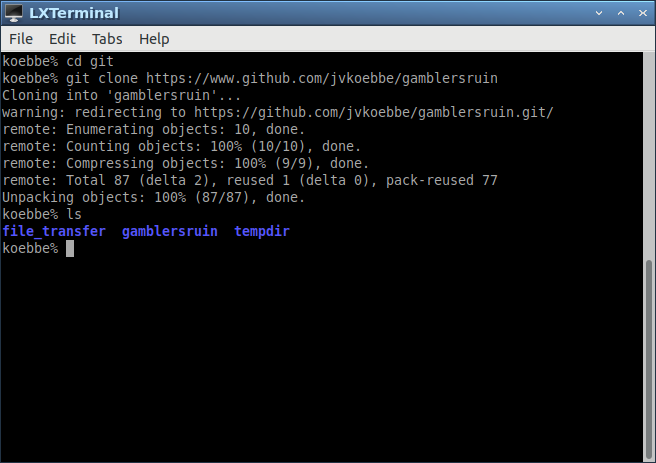
\includegraphics{../images/git_05.png}
\vskip0.1in
\caption{Creation of a local repository using the git clone command.}
\end{figure}
\eject
%%%%%%%%%%%%%%%%%%%%%%%%%%%%%%%%%%%%%%%%%%%%%%%%%%%%%%%%%%%%%%%%%%%%%%%%%%%%%%%%
%%%%%%%%%%%%%%%%%%%%%%%%%%%%%%%%%%%%%%%%%%%%%%%%%%%%%%%%%%%%%%%%%%%%%%%%%%%%%%%%
\vskip0.1in\hrule\vskip0.1in\noindent
{\bf Using the git status Command} 
\vskip0.1in\hrule\vskip0.1in\noindent
One of the most used commands in git is the status command. This will tell you
about any changes that have been made. For example,
\begin{verbatim}

    koebbe% git status

\end{verbatim}
You will use this command over and over if you are being efficient. An example
of the output is shown in the next figure when working in repository.
\vfill
\begin{figure}[h]
\centering
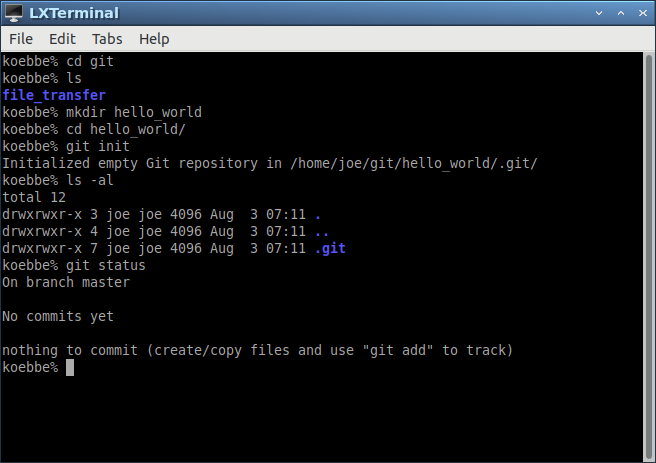
\includegraphics{../images/git_06.png}
\vskip0.1in
\caption{Using the git status command to List Changes.}
\end{figure}
\eject



%%%%%%%%%%%%%%%%%%%%%%%%%%%%%%%%%%%%%%%%%%%%%%%%%%%%%%%%%%%%%%%%%%%%%%%%%%%%%%%%
%%%%%%%%%%%%%%%%%%%%%%%%%%%%%%%%%%%%%%%%%%%%%%%%%%%%%%%%%%%%%%%%%%%%%%%%%%%%%%%%
\vskip0.1in\hrule\vskip0.1in\noindent
{\bf The git commit Command} 
\vskip0.1in\hrule\vskip0.1in\noindent

\vfill
\begin{figure}[h]
\centering
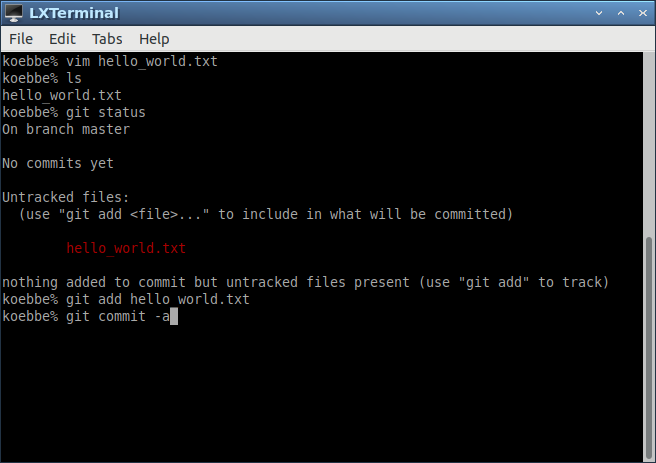
\includegraphics{../images/git_07.png}
\caption{{Screenshot} taken using {\bf Snip \& Sketch}. This is an app on
         my Windows 10 box}
\end{figure}
\eject


%%%%%%%%%%%%%%%%%%%%%%%%%%%%%%%%%%%%%%%%%%%%%%%%%%%%%%%%%%%%%%%%%%%%%%%%%%%%%%%%
%%%%%%%%%%%%%%%%%%%%%%%%%%%%%%%%%%%%%%%%%%%%%%%%%%%%%%%%%%%%%%%%%%%%%%%%%%%%%%%%
\vskip0.1in\hrule\vskip0.1in\noindent
{\bf The git push Command} 
\vskip0.1in\hrule\vskip0.1in\noindent

\vfill
\begin{figure}[h]
\centering
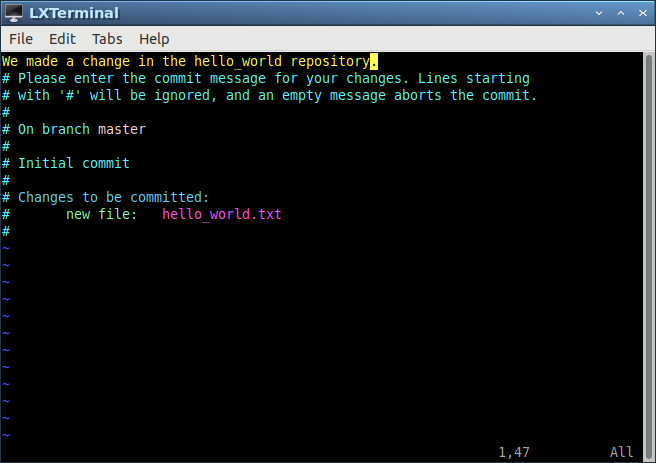
\includegraphics{../images/git_08.png}
\caption{{Screenshot} taken using {\bf Snip \& Sketch}. This is an app on
         my Windows 10 box}
\end{figure}
\eject



%%%%%%%%%%%%%%%%%%%%%%%%%%%%%%%%%%%%%%%%%%%%%%%%%%%%%%%%%%%%%%%%%%%%%%%%%%%%%%%%
%%%%%%%%%%%%%%%%%%%%%%%%%%%%%%%%%%%%%%%%%%%%%%%%%%%%%%%%%%%%%%%%%%%%%%%%%%%%%%%%
\vskip0.1in\hrule\vskip0.1in\noindent
{\bf The git pull Command} 
\vskip0.1in\hrule\vskip0.1in\noindent




\vfill
\begin{figure}[h]
\centering
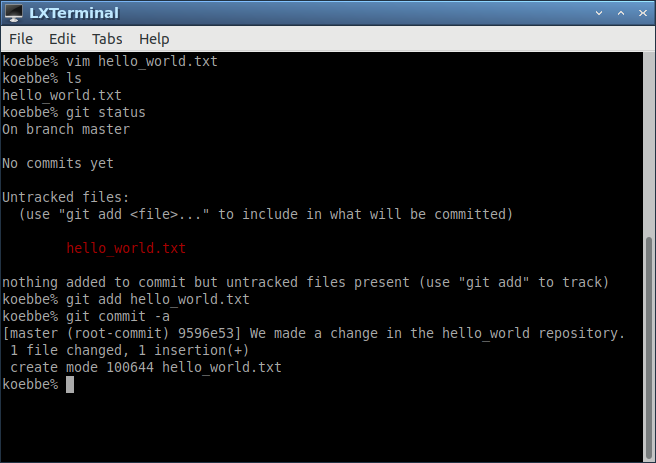
\includegraphics{../images/git_09.png}
\caption{{Screenshot} taken using {\bf Snip \& Sketch}. This is an app on
         my Windows 10 box}
\end{figure}
\eject
%%%%%%%%%%%%%%%%%%%%%%%%%%%%%%%%%%%%%%%%%%%%%%%%%%%%%%%%%%%%%%%%%%%%%%%%%%%%%%%%
%%%%%%%%%%%%%%%%%%%%%%%%%%%%%%%%%%%%%%%%%%%%%%%%%%%%%%%%%%%%%%%%%%%%%%%%%%%%%%%%
\end{document}
